% Journal-length draft on the Protective-Field Barrier (PFB). Generic single-column preprint layout
% (article class, natbib, no publisher template). Build: pdflatex, bibtex, pdflatex x2 (README.md).
% SCOPE (researcher, 2026-11-07): the full study -- classical planners and the learned (SAC) arms.
% BINDING RULES (supervisor, 2026-11-07): draft only, never submitted by anyone but the authors; every
% number is DEVELOPMENT-SET (tune set); held-out results are placeholders (\pending); learned arms are
% PILOT results; "B6 and B7 are indistinguishable at 3 vs 3 events"; "H1prime is a declared exploratory
% contingency; held-out evaluation pending". Every number is traced in README.md.
\documentclass[11pt]{article}
\usepackage[a4paper,margin=1in]{geometry}
\usepackage[T1]{fontenc}
\usepackage{lmodern}
\usepackage{microtype}
\usepackage{amsmath,amssymb,amsthm}
\usepackage{graphicx}
\usepackage{booktabs}
\usepackage{tabularx}
\usepackage{xcolor}
\usepackage{enumitem}
\usepackage[numbers,sort&compress]{natbib}
\usepackage{fancyhdr}
\usepackage[hidelinks]{hyperref}
\usepackage{caption}
\usepackage[section]{placeins}
\captionsetup{font=small,labelfont=bf}
\graphicspath{{figures/}}
\setlist{itemsep=2pt,topsep=4pt}

\newcommand{\pending}[1][held-out: pending]{\textcolor{red}{[#1]}}
\newcommand{\tbd}[1]{\textcolor{red}{[#1]}}
\newcommand{\dev}{\textsuperscript{\textsc{dev}}}
\newcommand{\Hprime}{H1$'$}
\theoremstyle{definition}
\newtheorem{definition}{Definition}

\pagestyle{fancy}
\fancyhf{}
\renewcommand{\headrulewidth}{0.4pt}
\fancyhead[L]{\small\textsc{Draft preprint} --- not submitted; development-set results only}
\fancyhead[R]{\small Kahoul and Kiram}
\fancyfoot[C]{\small\thepage}

\title{\textbf{Protective-Field Barriers: Control Barrier Functions\\ Consistent with Certified Safety Fields for Classical\\ and Learned Local Planners of Industrial Mobile Robots}}
\author{Mahdi Kahoul \qquad Firas Mohamed Elamine Kiram\\[2pt]
\small AMCO Laboratory, Padua, Italy\\
\small \texttt{mahdi.kahoul@univ-biskra.dz}}
\date{\small Draft of 7 November 2026. Not submitted; submission is the authors' decision.}

\begin{document}
\maketitle
\thispagestyle{fancy}

\begin{abstract}
\noindent Industrial autonomous mobile robots are protected by a certified safety function: safety laser
scanners monitor speed-dependent protective fields and command a latched protective stop whenever an
object enters the active field. The navigation software above this function does not model these fields,
so local planners, whether hand-designed or learned, trigger stops frequently, and every stop costs a
restart and throughput. This article introduces the Protective-Field Barrier (PFB), a discrete-time
control barrier function defined on the sectors of the laser scan, whose safe set is the complement of
the certified function's own trigger set. Its zero level set is a continuous protective field that
depends on the robot's footprint, speed, direction of travel and yaw rate, built from the same
configuration as the safety function. One quadratic program per speed regime minimally modifies the
command of an arbitrary planner, within the wheel-speed and acceleration limits of a holonomic base, and
falls back to maximal braking when no regime is feasible. We describe a study in which an emulated
certified layer runs beneath every controller, protective stops per 100\,m of planned route are the
primary endpoint, and hypotheses, comparators and analysis were preregistered. On the development
(tuning) set of 60 warehouse scenarios, placing the PFB beneath a tuned Regulated Pure Pursuit planner
reduces protective stops from 52.8 to 0.47 per 100\,m planned and the time spent latched from 42\,\% to
0.05\,\%, without reducing the planner's driving speed; a field-aware MPPI planner and the filtered planner
are indistinguishable at 3 versus 3 events. A Soft Actor-Critic planner trained with the PFB in the loop
passed its pilot gate on one pilot seed (0.95 stops per 100\,m planned, success 0.52), whereas a planner
trained with proximity shaping and no filter failed the gate on three pilot seeds. The comparison of the
filtered classical planner with the classical references is a declared exploratory contingency
hypothesis; the confirmatory comparisons and every held-out result are pending.
\end{abstract}

\noindent\textbf{Keywords:} control barrier functions; safety filters; safety laser scanners; protective
fields; local planning; safe reinforcement learning; autonomous mobile robots.

\vspace{4pt}
\noindent\fbox{\parbox{\dimexpr\linewidth-2\fboxsep-2\fboxrule}{\small\textbf{Status of the evidence.}
Every number in this draft is a \emph{development-set} result, obtained on the tuning set used to select
parameters, and is marked as such. Learned-planner results are \emph{pilot} results from pilot-range seeds
that never enter the confirmatory analysis. The held-out test evaluation has not been run; its tables
carry \pending\ placeholders. The comparison of the filtered classical planner with the classical
references (\Hprime) is a declared exploratory contingency; held-out evaluation pending.}}

%=====================================================================================================
\section{Introduction}\label{sec:intro}

Autonomous mobile robots (AMRs) move material through warehouses and factories in aisles they share
with people. Their safety does not rest on the navigation software. Industrial standards require a
certified safety function, independent of navigation, that detects persons and obstacles and stops the
vehicle \citep{iso3691-4,iso13849-1}. In practice this function is realised by safety laser scanners
qualified as electro-sensitive protective equipment \citep{iec61496-3}, which monitor a \emph{protective
field} around the vehicle. Because the stopping distance grows with speed, integrators configure several
fields and switch between them according to the vehicle's speed and direction of travel. An object inside
the active field triggers a protective stop, which latches until the field is clear and a restart
condition is met.

The navigation system above this layer, typically a global planner on a map and a local planner that
tracks the planned route, is neither certified nor aware of the protective fields. Classical local
planners represent obstacles by an inflation radius, a clearance term or a cost map
\citep{fox1997dwa,macenski2023rpp,williams2017mppi}, and learned local planners by a collision penalty
and proximity shaping in the reward \citep{le2024review,taheri2024ppo,cai2025agv}. None of these
corresponds to the field the scanner monitors: deeper in the direction of travel, larger at higher
speed, tied to the vehicle's footprint, and swept by the rotation the vehicle can make before it stops.
A planner that is collision-free in its own model therefore still enters the protective field at shelf
corners, in narrow aisles and near obstacles that are absent from the map. Each entry is a stop, a
restart delay and, in the worst case, a deadlock in which the restart condition never clears. On a
certified vehicle the collision rate, the usual safety metric of the navigation literature, is largely
bounded by the certified layer itself; the operational cost that remains is the protective stop.

Control barrier functions (CBFs) render a set forward invariant by constraining the input at every
state \citep{ames2017cbfqp,ames2019cbf}; used as a safety filter, a small quadratic program (QP) selects
the admissible input closest to the command of an unmodified upstream controller
\citep{wang2022ensuring,wabersich2023safety}. In mobile robotics the safe set of such filters is a
clearance to observed points or obstacles, sometimes inflated with the relative velocity
\citep{raja2024ogmcbf,zeng2025relvel}. That clearance is chosen by the designer and bears no explicit
relation to the certified field: a filter with too small a clearance still triggers stops, and one with
too large a clearance stops the robot by itself.

This article proposes to take the safe set of the barrier from the certified safety function: every
valid scan return must lie outside the protective field of the regime the robot will be in. The barrier
is then exactly as conservative as the equipment it sits above, no more and no less, and its success can
be measured in the units in which the equipment charges for failure: protective stops. The contributions
are as follows.
\begin{itemize}
\item \textbf{The Protective-Field Barrier.} A discrete-time CBF defined per sector of the laser scan,
whose zero level set is a continuous protective field built from the measured footprint and the
certified configuration: the motion reachable within the safety function's reach time followed by
braking, the lateral swerve an acceleration limiter permits, the rotation swept while stopping, and the
drift of a body that turns while it translates (Section~\ref{sec:pfb}).
\item \textbf{A filter for a holonomic base.} One QP per speed regime of the certified layer, with the
mecanum wheel-speed polytope, the axis box and the acceleration limiter's one-step envelope as
constraints, linearised about a reachable command, checked against the exact barrier rows and falling
back to maximal braking; and a rule that passes, under a latched stop, only commands the restart
condition could release.
\item \textbf{An evaluation that includes the safety layer.} An emulated certified layer with
speed-banded fields and latched stops, implemented independently of the filter, runs beneath every
controller, classical and learned; the primary endpoint is protective stops per 100\,m of planned route;
hypotheses, comparators, gates and the analysis (a two-level interval on the rate ratio) were
preregistered, and every later change was recorded by dated amendment (Section~\ref{sec:design}).
\item \textbf{Development-set and pilot evidence}, reported with its limits: the filter beneath a
classical planner, five tuned classical references, the pilot gates of the learned planners and
diagnostics of their behaviour (Section~\ref{sec:results}).
\end{itemize}

Section~\ref{sec:related} reviews related work, Section~\ref{sec:problem} formulates the problem,
Section~\ref{sec:pfb} derives the barrier and the filter, Section~\ref{sec:design} describes the system
and the experimental design, Section~\ref{sec:results} reports the development-set and pilot results,
Section~\ref{sec:discussion} discusses them with their limitations, and Section~\ref{sec:conclusion}
concludes.

%=====================================================================================================
\section{Related Work}\label{sec:related}

\subsection{Industrial safety standards and protective fields}
Driverless industrial trucks are governed by ISO~3691-4 \citep{iso3691-4}. Personnel detection is
commonly provided by safety laser scanners qualified under IEC~61496-3 \citep{iec61496-3}, and the
selection of a field set according to speed and direction is itself a safety function, implemented in a
safety controller that must reach a required performance level \citep{iso13849-1}. The protective field
must contain the vehicle's stopping travel from the moment of detection, including the response time of
the scanner and the controller; it is sized at commissioning from measured stopping distances, with a
supplement for measurement error. A protective stop latches, and a restart requires the field to be
clear, either automatically after a delay or by an operator reset. The standards prescribe the
behaviour of this layer; they do not prescribe how the navigation software should avoid triggering it.
Barrier functions derived from standard-mandated stopping requirements have recently been proposed for
collaborative manipulators~\tbd{citation withheld until its authors are verified: arXiv:2606.13203, bib key iso10218cbf2026}; we are not aware of a comparable construction for
mobile bases.

\subsection{Classical local planners}
Pure Pursuit \citep{coulter1992purepursuit} steers towards a lookahead point on the route. Regulated
Pure Pursuit (RPP) \citep{macenski2023rpp}, the default path tracker of the Nav2 framework
\citep{macenski2020nav2}, additionally reduces speed with path curvature and with the proximity of
obstacles. The Dynamic Window Approach \citep{fox1997dwa} samples velocities reachable within one
acceleration window and scores their short trajectories for progress, heading and clearance. Model
Predictive Path Integral control (MPPI) \citep{williams2017mppi} optimises a control sequence by
importance-weighting sampled rollouts and admits arbitrary, even discontinuous, costs; it can therefore
carry the certified field in its cost, which makes it the natural hand-designed competitor of a
field-consistent filter. In all four the obstacle model is a clearance or a cost chosen by the designer;
none treats the protective field as a hard constraint.

\subsection{Control barrier functions and safety filters}
For a control-affine system and a safe set $\mathcal{C}=\{x: h(x)\ge 0\}$, the condition
$\dot h(x,u)\ge-\alpha(h(x))$, with $\alpha$ an extended class-$\mathcal{K}$ function, renders
$\mathcal{C}$ forward invariant, and because it is affine in $u$ the closest admissible input is the
solution of a QP \citep{ames2017cbfqp,ames2019cbf}. Its discrete-time counterpart,
$h(x_{k+1})\ge(1-\gamma)h(x_k)$ with $\gamma\in(0,1]$, is the form used on sampled systems
\citep{agrawal2017discrete}. Safety filters built on this principle correct the commands of learned
motion planners \citep{wang2022ensuring}, are constructed from the policy at run time
\citep{knoedler2025onthefly}, or are combined with predictive and reachability-based filters
\citep{wabersich2023safety}. Shielding restricts a controller's actions according to a formal
specification \citep{alshiekh2018shielding}. On mobile robots, the barrier is usually a distance to
points of a scan or an occupancy grid \citep{raja2024ogmcbf}, possibly inflated with the relative
velocity of nearby agents \citep{zeng2025relvel}; the footprint and the geometry of the stopping manoeuvre
enter only through margins. The PFB belongs to this family but changes the safe set: rather than a
clearance of the designer's choosing, it is the region whose violation the certified function punishes,
evaluated at the speed, direction and yaw rate the robot can reach.

\subsection{Safe and constrained reinforcement learning for navigation}
Deep reinforcement learning maps range observations to velocity commands with off-policy actor-critic
methods such as Soft Actor-Critic (SAC) \citep{haarnoja2018sac} and TD3 \citep{fujimoto2018td3};
hierarchical designs give a learned local policy the waypoints of a classical global planner
\citep{zhu2023hierarchical,kolomeytsev2025hybrid}. Safety is then addressed in three ways. The most common
encodes it in the reward through collision penalties and proximity shaping
\citep{taheri2024ppo,cai2025agv,li2024warehouse}, which offers no guarantee and makes the safety term
compete with the task. Constrained formulations bound an expected cost within a constrained Markov
decision process \citep{altman1999cmdp}, solved by trust-region \citep{achiam2017cpo} or Lagrangian
methods \citep{ray2019benchmarking}; PID control of the Lagrange multiplier damps the oscillations of
plain dual ascent \citep{stooke2020pid}. Run-time enforcement filters the policy's actions: CBF-QP
filters have been placed beneath navigation policies \citep{guo2025radar}, the barrier's gain has been
adapted by the policy \citep{mohammad2025sacadapt}, and filters applied during training let the policy
learn from filtered transitions \citep{cheng2019endtoend,yang2025cbfrl}. Evaluation practice varies
widely, and single-seed results remain common despite the variance between seeds that deep RL is known
to exhibit \citep{henderson2018matters,agarwal2021precipice}. The present study trains with the filter in
the loop and keeps it at deployment, compares against shaped, constrained and post-hoc-filtered
alternatives, and treats the training seed as a unit of analysis.

%=====================================================================================================
\section{Problem Formulation}\label{sec:problem}

\begin{figure}[!htbp]
\centering
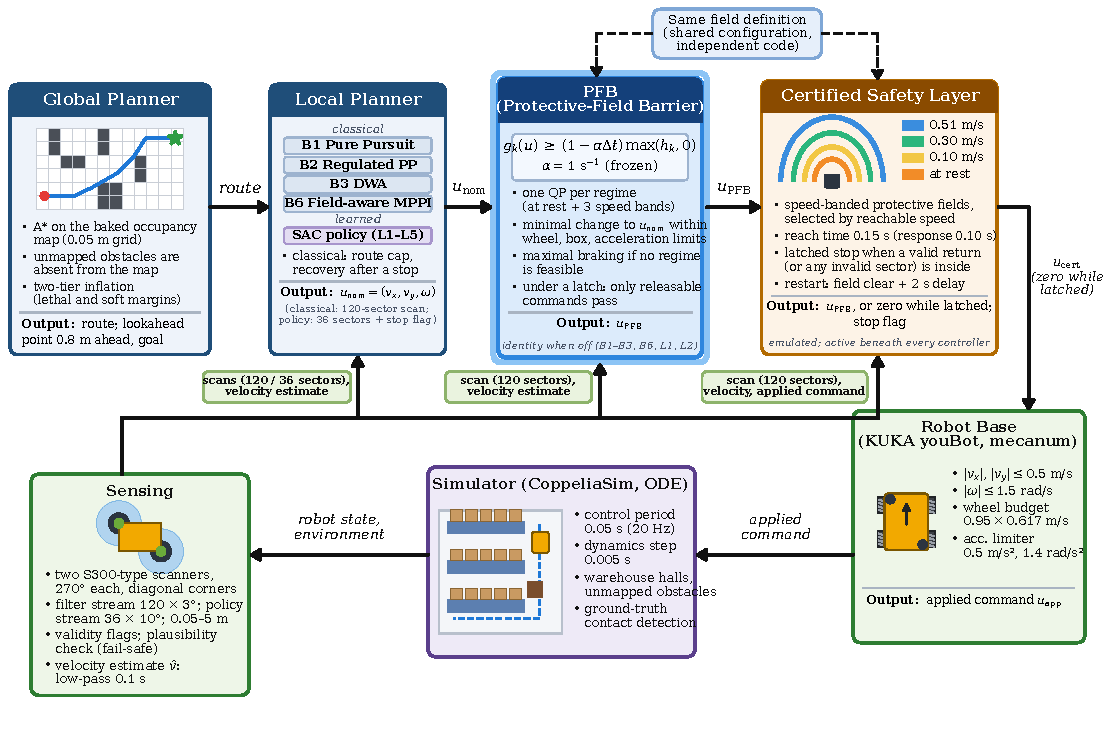
\includegraphics[width=\textwidth]{fig_architecture.pdf}
\caption{System architecture. Every controller, learned or classical, sends its command through the
same path: the PFB slot (the identity when the filter is off), the certified-layer emulator, which
decides on the scan already in hand and replaces the command by zero while a protective stop is latched,
and the base's velocity box, wheel-speed budget and acceleration limiter. The policy receives the
36-sector policy stream; the PFB, the certified layer and the classical planners receive the 120-sector
filter stream with measured bearings and validity flags.}
\label{fig:arch}
\end{figure}

Figure~\ref{fig:arch} shows the system. A global planner supplies a route on a map that omits some
obstacles; a local planner proposes a body-frame velocity command; the PFB filters it; an emulated
certified layer, active beneath every controller, may override any command with a latched stop; and the
base applies what remains through its kinematic limits. All quantities are in SI units in the body frame
($+x$ forward, $+y$ left, bearings in $(-\pi,\pi]$); the notation is collected in
Appendix~\ref{app:notation}.

\subsection{Holonomic platform and actuation}
The platform is a four-wheel mecanum base derived from the KUKA youBot, commanded by a body twist
$\mathbf{u}=(v_x,v_y,\omega)$ at a control period $\Delta t=0.05$\,s. Its footprint is not a datasheet
rectangle but a measured table $e(\psi)$, the distance from the body origin to the envelope of every part
that can strike an obstacle (chassis, wheels and scanner housings) along each bearing, obtained with a
collision probe in the simulator. Its inscribed and circumscribed radii are 0.209\,m and
$\rho_{\mathrm{out}}=0.3374$\,m. Measured values are configured at the upper bound of their measurement
bracket, since under-stating a safety footprint is the unsafe direction.

By the mecanum mixing, the fastest wheel's rim speed is $|v_x|+|v_y|+L|\omega|$, with lever arm
$L=0.3865$\,m (half wheelbase plus half track), and the wheel-speed limit is the polytope
\begin{equation}
|v_x|+|v_y|+L|\omega|\le f\,v_{\mathrm{rim}},
\label{eq:budget}
\end{equation}
where $v_{\mathrm{rim}}=0.617$\,m/s is the measured rim-speed ceiling and the share $f=0.95$ applies to
the filter's output and the base's final ceiling. An axis box $|v_x|,|v_y|\le0.5$\,m/s,
$|\omega|\le1.5$\,rad/s sits inside the budget; commands outside either are scaled along their own
direction. An acceleration limiter bounds every change of the applied command:
\begin{equation}
\big\|(v_x,v_y)_k-(v_x,v_y)_{k-1}\big\|\le
\begin{cases}a_{\mathrm{dec}}\Delta t & \text{if the planar speed decreases},\\ a_{\max}\Delta t &
\text{otherwise},\end{cases}\qquad |\omega_k-\omega_{k-1}|\le\alpha_{\max}\Delta t,
\label{eq:limiter}
\end{equation}
with $a_{\max}=0.5$\,m/s$^2$, $a_{\mathrm{dec}}=1.0$\,m/s$^2$ and $\alpha_{\max}=1.4$\,rad/s$^2$. These
bounds are not properties of the youBot: they are co-specified with the protective fields, so that no
speed band can be skipped within one reach time and no controller can brake harder than the fields
assume. The safety layers use the estimated actual body velocity $\hat{\mathbf{v}}$, from differenced
poses low-pass filtered with a time constant of 0.10\,s.

\subsection{Scanner model}
Two scanners of the SICK S300 type sit on diagonally opposite corners, each covering 270$^\circ$, so that
together they see everything outside the outline; this layout replaced the platform's original
centreline sensors after verification found a blind zone beside the robot inside the protective field
(Appendix~\ref{app:verification}). The scan plane lies 0.2206\,m above the floor. The returns are binned
in the simulator into two streams: a \emph{policy stream} of 36 sectors of 10$^\circ$, and a \emph{filter
stream} of 120 sectors of 3$^\circ$, each carrying the minimum range $r_k\in[0.05,5.0]$\,m, the bearing
$\psi_k$ at which it was measured and a validity flag $\chi_k$. A sector is valid only if its whole
extent, from the footprint edge to 1.0\,m beyond it, is seen by some sensor from where that sensor is.
\emph{Unobserved space is never treated as free}: an invalid sector breaches every certified field, and
the PFB and the classical planners treat it as an obstacle at the footprint boundary. A plausibility
check against the previous scan, with re-rendering and a fail-safe, guards against corrupted frames under
load (Appendix~\ref{app:verification}).

\subsection{The certified layer}\label{sec:certified}
The certified layer is emulated as a scanner with switchable field sets and a safety controller that
selects the set and latches stops. It is implemented independently of the PFB, with which it shares
configuration keys but no code, and it runs beneath every controller. It emulates the behaviour of such
equipment; it makes no claim of functional-safety compliance.

\paragraph{Containment and reach time.} The field in force when a stop triggers must contain everything
the footprint sweeps until the robot is at rest. During the response time $t_r=0.10$\,s the command still
passes and may keep accelerating, so fields are sized over the \emph{reach time}
$T=t_r+\Delta t=0.15$\,s, followed by braking at $a_b=1.0$\,m/s$^2$ in translation and $\alpha_{\max}$ in
rotation.

\paragraph{Speed bands.} The field set is selected by the \emph{reachable} speed: with $s$ the composed
planar speed,
\begin{equation}
\bar v(s)=\max\big(s,\min(s+a_{\max}T,\,v_{\mathrm{cap}})\big),\qquad
\ell(s)=\min\{\ell:\bar v(s)\le V_\ell\},
\label{eq:band}
\end{equation}
with band tops $V_\ell\in\{0.10,0.30,0.51\}$\,m/s and $v_{\mathrm{cap}}=0.5074$\,m/s the largest
planar speed the box and the budget allow. Since $a_{\max}T=0.075$\,m/s is below the narrowest band
width, no band can be skipped within one reach time.

\paragraph{Field geometry.} Each field is a convex set given by its support function. For travel at
direction $\theta$ in a band topped at $V$, with yaw rate $\omega$, normal angle $n$, $c=\cos(n-\theta)$
and $c^+=\max(0,c)$,
\begin{equation}
\begin{aligned}
h_V(n;\theta,\omega)=\max\Big(&S\big(n;E(|\omega|)+E(0)\big)+\max\big(D(V)c^+,\sigma(c,V)\big)+K(V,\omega)\\
&+\max\big((m_f-m_l)c^+,R\big)+m_l,\;\;h_{\mathrm{rest}}(n;\omega)\Big),
\end{aligned}
\label{eq:field}
\end{equation}
and the at-rest field is $h_{\mathrm{rest}}(n;\omega)=S\big(n;E(|\omega|)\big)+R+m_l$. Here
$S(n;\varepsilon)$ is the support of the footprint rotated through every heading in
$[-\varepsilon,\varepsilon]$; $E(\omega)$ is the heading change reachable from yaw rate $\omega$ within $T$
and then braking ($E(0)=0.0315$\,rad); $D(V)=VT+V^2/(2a_b)$ is the travel along the direction of motion;
$\sigma$ is the displacement off that direction that an isotropic limiter allows; $K(V,\omega)=D(V)\cdot
2\sin\big(\tfrac12\min(E(|\omega|),\pi)\big)$ bounds the drift of a body whose velocity turns with it;
$R=0.0131$\,m is the reach from the fastest speed still classified as at rest; and $m_f=0.10$\,m and
$m_l=0.05$\,m are the margins ahead and abeam. The boundary distance along a bearing $\psi$ is
\begin{equation}
\rho(\psi)=\min_{n:\cos(\psi-n)>0}\frac{h(n)}{\cos(\psi-n)},
\label{eq:extent}
\end{equation}
evaluated over 1{,}440 normals. Three properties hold by construction: the at-rest field is the infimum
of the moving fields, so the field never shrinks as speed rises; a stop that begins in motion ends with
the at-rest field inside the field in force at the trigger (nesting); and rotation enters both through the
sweep $S$ and through $K$. Figure~\ref{fig:field} shows the fields.

\begin{figure}[!htbp]
\centering
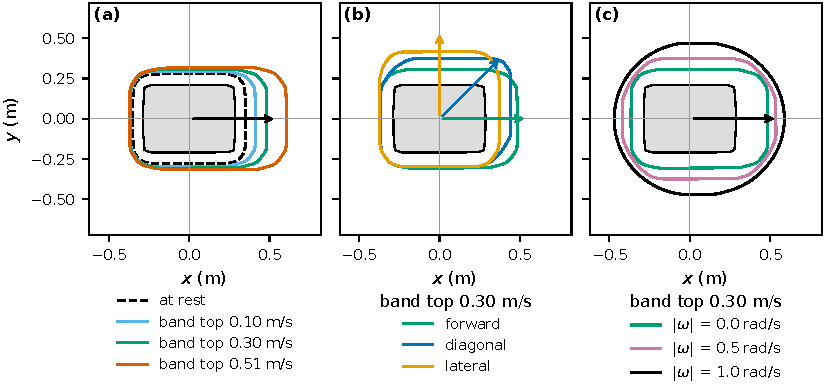
\includegraphics[width=\textwidth]{fig2_field_geometry.pdf}
\caption{Protective fields from \eqref{eq:field}--\eqref{eq:extent} on the measured footprint (grey).
(a) The at-rest field and the three band fields for straight forward travel. (b) The band-1 field for
forward, diagonal and lateral travel. (c) The band-1 field for forward travel at three yaw rates, showing
the rotation sweep and the turning-drift term.}
\label{fig:field}
\end{figure}

\paragraph{The field in force.} The layer never sizes the field below true motion. Its composed speed is
$s=\max(\|\hat{\mathbf{v}}_{xy}\|,\|\mathbf{u}^{\mathrm{app}}_{xy}\|)$, the larger of the estimated
speed and that of the command the base is executing, and its yaw rate whichever of $\hat\omega$ and
$\omega^{\mathrm{app}}$ is larger in magnitude: the command alone understates motion while
decelerating, the lagged estimate while accelerating. A standstill detector with hysteresis classifies
the robot as at rest (entry below 0.01\,m/s and 0.0296\,rad/s, exit above 0.02\,m/s or 0.0592\,rad/s);
the field in force is $h_{\mathrm{rest}}$ at rest and $h_{V_{\ell(s)}}$ otherwise.

\paragraph{Breach, latch and restart.} A valid return inside the field in force ($r_k<\rho(\psi_k)$), or
any invalid sector, is a breach. A breach while no stop is pending triggers a protective stop, which
becomes active $t_r$ later; from then on every command is replaced by zero. The stop holds while the field
is breached and for a restart delay $t_d=2.0$\,s after it last came clear. Release then requires the whole
field of the commanded twist to be clear, the commanded translation to have no component toward any
breaching point, and the velocity of the footprint point nearest each breaching point to have no
component toward it. A creep regime, slow enough to keep the at-rest field, is the way out of the thin
shell that containment and nesting leave around a stopped robot; a robot held at rest with its own
at-rest field breached is released, after $t_d$, only for a creep under which every point inside that
field strictly recedes (the \emph{receding release}), which is less conservative than the operator reset
of real equipment. A larger warning field is counted as a near-miss metric and never acts.

\subsection{Navigation stack}
Each layout is rasterised into a 0.05\,m planner grid from which obstacles absent from the map are
excluded. Cells within the inscribed half-width plus 0.10\,m (0.3086\,m) of an obstacle are lethal; a soft
cost falls linearly from the lethal radius to the circumscribed radius plus 0.03\,m. An 8-connected A*
search with the octile heuristic finds the cheapest path, simplified by line of sight. Progress is the
arc length of the robot's monotonic projection onto the route, and the controller is given a lookahead
point 0.8\,m of arc ahead and the goal, in the body frame. The stack does not replan.

\subsection{Definitions and the primary metric}\label{sec:defs}
\begin{definition}[Protective stop]
A trigger event of the certified layer: a step at which the field in force is breached while no stop is
triggered or latched. A persisting breach and the latched stop that follows it count once.
\end{definition}
\begin{definition}[Scan-fault stop]
A protective stop decided on a packet that failed the plausibility check through every re-render and was
replaced by the fail-safe. Excluded from the primary count and reported beside it.
\end{definition}
\begin{definition}[Contact]
Decided by the simulator's collision check alone, chassis and housings against every object outside the
robot including the floor, wheels against the same set without the floor. Range readings never define a
collision.
\end{definition}
\begin{definition}[Unrecoverable stop]
An episode that reaches its horizon while a stop is latched and the robot cannot legally move again;
distinguished from a timeout, in which the robot was free to move.
\end{definition}

The primary endpoint is the number of protective stops per 100\,m of \emph{planned} route, pooled over
episodes:
\begin{equation}
\mathrm{SP100}=100\,\frac{\sum_e\big(N^{\mathrm{stop}}_e-N^{\mathrm{fault}}_e\big)}{\sum_e L_e},
\label{eq:sp100}
\end{equation}
where $L_e$ is the length of episode $e$'s planned route. The planned length is a property of the
scenario, identical for every controller, so a controller cannot lower its rate by driving further; an
earlier version divided by the distance driven, which was moved to a secondary endpoint before any test
data existed, once a learned planner was observed to drive 1.6 times its routes
(Section~\ref{sec:res-learned}). Stops per 100\,m driven, per 100\,m on completed routes only, the success
rate, mission time, the share of time latched and the \emph{moving speed} (mean speed while not latched)
are reported beside it.

\paragraph{Problem.} Given an arbitrary nominal command $\mathbf{u}^{\mathrm{nom}}$, the scan and the
velocity estimate, find at every step the admissible command closest to $\mathbf{u}^{\mathrm{nom}}$ under
which the certified layer does not trigger, so that the robot reaches its goal within the horizon, without
contact, with as few protective stops per 100\,m of planned route as possible.

%=====================================================================================================
\section{The Protective-Field Barrier}\label{sec:pfb}

The PFB is a safety filter between the planner and the certified layer. It reads the same scan, velocity
estimate and applied command as the certified layer and builds its field from the same configuration
keys, through its own implementation; the two are cross-checked only in tests. Throughout,
$\mathbf{u}^{\mathrm{nom}}$ is the planner's command and $\mathbf{u}^-$ the command the base applied at
the previous step.

\subsection{Regimes and the per-sector barrier}
The certified layer is in one of four regimes $\lambda\in\Lambda=\{\mathrm{rest},0,1,2\}$: at rest, or
moving in one of the three bands. Because the band is chosen from the reachable speed and switches
discretely, the PFB solves one problem per regime and keeps the best feasible answer; its field in
regime $\lambda$, $\rho_\lambda(\psi;\theta,W)$, is \eqref{eq:extent} built from $h_{\mathrm{rest}}$ or
from $h_{V_\lambda}$. For a valid sector $k$ with return $\mathbf{p}_k=r_k(\cos\psi_k,\sin\psi_k)$, the
barrier is the distance of the return outside the field,
\begin{equation}
h^\lambda_k=r_k-\rho_\lambda(\psi_k;\theta_0,W_0)-\delta,
\label{eq:barrier}
\end{equation}
evaluated at the present motion ($\theta_0$ the heading of whichever of $\mathbf{u}^-$ and
$\hat{\mathbf{v}}$ is faster, $W_0=\max(|\hat\omega|,|\omega^-|)$), where $\delta=0.5$\,mm is the
measured scan residual against a wall face at the upper bound of its bracket. The safe set of regime
$\lambda$ is $\{h^\lambda_k\ge0\ \forall k\}$: the complement of the certified trigger set in that regime.

\subsection{Prediction and the discrete-time barrier condition}
A candidate command moves each return relative to the body. Over the horizon $\tau=\Delta t+\tau_\ell$,
one control step plus a declared lag allowance $\tau_\ell=0.05$\,s, a return is predicted at
\begin{equation}
\mathbf{p}'_k(\mathbf{u};\mu)=\mathbf{R}(-\mu\omega\tau)\big(\mathbf{p}_k-\mu\tau(v_x,v_y)\big),
\label{eq:prediction}
\end{equation}
where $\mu\in[0,1]$ is the fraction of the predicted motion realised so far. The predicted barrier is
\begin{equation}
g^\lambda_k(\mathbf{u};\mu)=\|\mathbf{p}'_k\|-\rho_\lambda\big(\angle\mathbf{p}'_k;\theta(\mathbf{u}),W(\mathbf{u})\big)-\delta,
\label{eq:predicted}
\end{equation}
in which the field faces the candidate's own direction of travel $\theta(\mathbf{u})=
\operatorname{atan2}(v_y,v_x)$ when its speed is at least the estimated speed, and the estimate's
otherwise, and is swept for $W(\mathbf{u})=\max(|\hat\omega|,|\omega|)$. As in the certified layer, the
field is never sized below the larger of estimated and commanded motion. The filter admits $\mathbf{u}$
in regime $\lambda$ only if, for every valid sector within reach,
\begin{equation}
\min_{\mu\in M}g^\lambda_k(\mathbf{u};\mu)-\epsilon_\mu\;\ge\;(1-\alpha\Delta t)\,\big[h^\lambda_k\big]^+,
\qquad M=\{0,\tfrac14,\tfrac12,\tfrac34,1\},
\label{eq:cbf}
\end{equation}
with class-$\mathcal{K}$ gain $\alpha$ and $[\cdot]^+=\max(\cdot,0)$. Requiring the row over the realised
fractions $M$, with a margin $\epsilon_\mu=0.5$\,mm that bounds the measured gap between the grid minimum
and the minimum over all $\mu\in[0,1]$, keeps the condition valid along the whole step rather than only at
its end. The clipped right-hand side departs deliberately from the standard discrete-time condition
$g\ge(1-\gamma)h$ \citep{agrawal2017discrete}. Within one regime the clearance may decay at most at rate
$\alpha$, as usual. Across regimes, however, the barrier of a field the robot is not yet in may already be
negative, and the standard form would then admit entering it as long as the violation shrank; since the
certified layer acts on the first breach, the clipped form requires a regime whose field is breached now
to be clear after one step, which in practice rules that regime out.

\subsection{The quadratic program}
For each admissible regime the filter seeks the admissible command closest to the nominal one:
\begin{equation}
\begin{aligned}
\min_{\mathbf{u}}\quad&(\mathbf{u}-\mathbf{u}^{\mathrm{nom}})^\top\operatorname{diag}(1,1,\rho_{\mathrm{out}}^2)\,(\mathbf{u}-\mathbf{u}^{\mathrm{nom}})\\
\text{s.t.}\quad&\eqref{eq:cbf}\ \text{for every valid sector, linearised},\\
&\eqref{eq:budget}\ \text{and the axis box},\\
&\text{the one-step envelope of \eqref{eq:limiter} about }\mathbf{u}^-,\\
&\|(v_x,v_y)\|\le\bar V_\lambda,\qquad|\omega|\le0.9\,\omega_{\mathrm{out}}\ \text{if}\ \lambda=\mathrm{rest}.
\end{aligned}
\label{eq:qp}
\end{equation}
The weight $\rho_{\mathrm{out}}^2$ makes one rad/s of turning cost what the footprint's outermost point
moves. The regime speed limit $\bar V_\lambda$ keeps the robot in its regime under reach: $V_\lambda-a_{\max}
T$ less 0.002\,m/s for bands 0 and 1, $v_{\mathrm{cap}}$ for the top band, and a creep speed of 0.018\,m/s
at rest. The limiter's envelope is non-convex, since it depends on whether the command slows down, and is
imposed as two convex cases solved in turn (holding or accelerating; braking without gaining speed), with
discs as inscribed 16-gons so that every feasible point is reachable.

\paragraph{Admissible regimes.} The rest regime is admissible only while a mirror of the standstill
detector classifies the robot as at rest; a band is admissible only if it is not below the band the
estimated speed selects, because the estimate lags. If $\mathbf{u}^{\mathrm{nom}}$ satisfies every
constraint and row of some admissible regime, it passes unchanged; otherwise every admissible regime is
solved and the feasible solution of least cost is applied.

\paragraph{Linearise, check, fall back.} The rows of \eqref{eq:cbf} are non-convex in $\mathbf{u}$. Each
regime's problem is linearised about a reachable point near $\mathbf{u}^{\mathrm{nom}}$ (the nominal step
from $\mathbf{u}^-$ clipped to the envelope, the regime's speed limit and the yaw box, then scaled into the
wheel polytope). In translation each row keeps its tangent. In the yaw rate, where the field grows
convexly with $|\omega|$ and has a kink at $|\hat\omega|$, each row is replaced by its two chords over a
trust interval of $\pm0.05$\,rad/s, which lie below the true row. The linearised rows are tightened by
0.5\,mm and rows with more than 0.5\,m of linearised slack are omitted. The QP is solved by an
interior-point method \citep{goulart2024clarabel}. A solution is accepted only if it satisfies every
\emph{true} row \eqref{eq:cbf} with no tolerance; otherwise the problem is linearised once more, about
that solution (or about the braking command if the first problem was infeasible). If no regime yields an
accepted solution, the filter applies maximal braking within the limiter,
\begin{equation}
(v_x,v_y)\leftarrow(v^-_x,v^-_y)\Big[1-\frac{a_{\mathrm{dec}}\Delta t}{\|(v^-_x,v^-_y)\|}\Big]^+,\qquad
\omega\leftarrow\operatorname{sgn}(\omega^-)\big[|\omega^-|-\alpha_{\max}\Delta t\big]^+,
\label{eq:fallback}
\end{equation}
which is labelled a feasible braking step if it satisfies the true rows of an admissible regime and a
\emph{fallback step} otherwise; fallback steps are counted per method and stratum.

\paragraph{Behaviour under the latch.} While the certified layer holds a stop, the filter passes only
commands that the restart condition could release (a creep whose at-rest field is clear or that strictly
recedes from every point inside it, or a faster twist whose own band field is clear) and replaces every
other command by zero. A planner's recovery creep therefore passes unaltered when it is releasable.

\paragraph{What the construction guarantees, and what it does not.} If the QP is feasible, the accepted
command satisfies the exact barrier rows of its regime at every realised fraction of the step, under the
model of \eqref{eq:prediction}: static returns, the declared lag, and a base that executes the filtered
command within its limiter. It does not guarantee the absence of stops. Moving or newly revealed
obstacles, prediction error from wheel slip and estimation lag, and states in which no regime is feasible
(for example an unmapped obstacle across a narrow route, where braking alone cannot keep the field clear)
all remain, and the certified layer beneath stays the safety function. The PFB is not a certified
component; its role is to make the certified function's interventions rare.

\begin{figure}[!htbp]
\centering
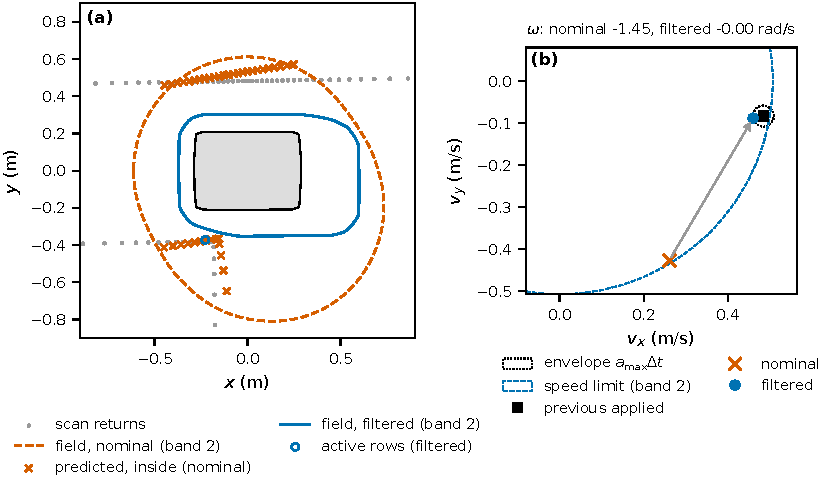
\includegraphics[width=\textwidth]{fig5_pfb_step.pdf}
\caption{One PFB step on a tuning route, from the emulator, at the step where the filter changed the
nominal command most. (a) Body frame: the scan returns and footprint, the field of the nominal command's
regime (dashed) with the returns predicted inside it, and the field of the filtered command (solid) with
its active rows. (b) The translational plane: the previous, nominal and filtered commands, the limiter's
envelope and the regime's speed limit. The nominal command is that of a scan-blind ideal route tracker.}
\label{fig:step}
\end{figure}

Figure~\ref{fig:step} illustrates one step: the nominal command would carry 40 returns into the predicted
field; the filter keeps most of the forward motion and removes the lateral and rotational components that
cause the violation. The PFB requires only the nominal command, the scan and the velocity estimate; the
planner is unchanged.

%=====================================================================================================
\section{System Architecture and Experimental Design}\label{sec:design}

\subsection{Simulator and architecture}
The experiments run in CoppeliaSim \citep{rohmer2013vrep} with the ODE engine at a dynamics step of
0.005\,s. The engine is a stated condition: in a declared sweep, the same model's heading drift on a 5\,m
lateral profile was 20.55$^\circ$ under Bullet, 0.47$^\circ$ under ODE and 3.12$^\circ$ under Newton.
Determinism is claimed within one scene load only; repetitions within a load are bit-identical, and
paired comparisons run their members within one load. The scanners are processed inside the simulator and
published as one packet per control step; the environment, filter, certified layer and controllers run in
Python. The environment's code is frozen by hash before any training, and every run records its commit,
host, scene hash, environment hash and resolved configuration.

\subsection{Layouts, clearance strata and obstacles absent from the map}
Each scenario is a procedurally generated warehouse hall with perimeter walls and two to four rows of
shelving taller than the scan plane (Figure~\ref{fig:layout}). Aisles are stratified by per-side
clearance, the gap on each side of a centred, aligned robot: narrow $[0.1987,0.2687)$\,m, medium
$[0.2687,0.40)$\,m and wide $[0.40,0.80]$\,m. The narrow floor follows a declared rule: the smallest
clearance at which the at-rest and moving fields of a robot displaced by the committed tracking bound
remain clear of the aisle walls on the 120-sector scan, plus a 0.03\,m buffer. Start and goal are drawn so
that at least 1.5\,m of the route lies in an aisle, and every route must be traversable by a
free-orientation oracle whose band-0 field stays clear from start to goal; on failure the goal, never the
layout, is re-drawn.

The central condition of the study is a world that differs from the map. Unmapped obstacles, square
boxes of 0.25--0.60\,m taller than the scan plane, are placed relative to the planned route: the first
at an offset uniform on $[0,0.3]$\,m from the route to its nearest surface, any second on $[0,0.6]$\,m.
An obstacle is kept only if the robot could pass it within $W=1.0$\,m of the route, judged jointly with
the obstacles already placed, since a stack that never replans cannot use a detour through another aisle.
The planner never sees these obstacles; the scanners and the safety layers do.

\begin{figure}[!htbp]
\centering
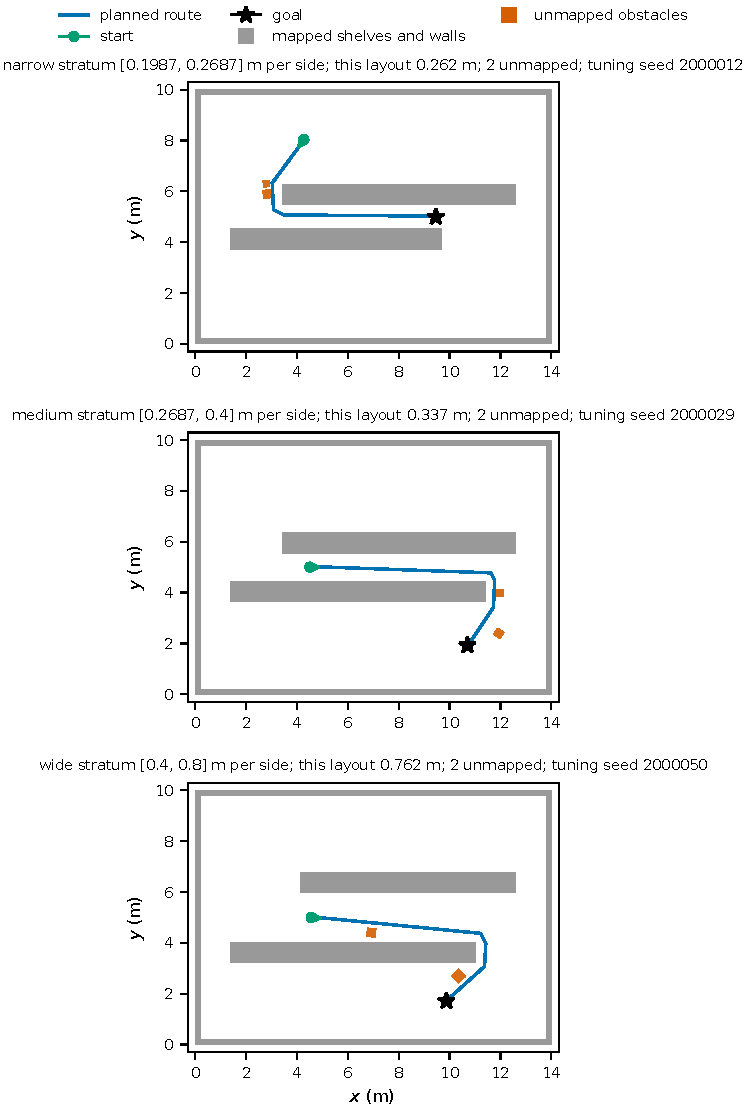
\includegraphics[width=0.62\textwidth]{fig4_layout.pdf}
\caption{Example layouts from the tuning set (never the test set), one per clearance stratum, with the
planned route, the shelf rows and the unmapped obstacles placed near the route.}
\label{fig:layout}
\end{figure}

\subsection{Scenario sets}
Layouts are identified by seed, geometry hash and generator hash, regenerated and verified at load, and
drawn from disjoint seed ranges for training, tuning, testing and piloting. The \emph{training set} holds
2{,}001 scenarios in equal thirds by stratum (mean planned length 10.67\,m), each training seed visiting it
in its own permutation shared by every method's seed of the same index. The \emph{tuning set}, the
development set of this article, holds 20 scenarios per stratum (60 in all, 633\,m planned) at an
unmapped-obstacle rate of 0.25; 17 of its 60 scenarios contain one or two unmapped obstacles. The
\emph{test set} has a mapped-only and an unmapped-static condition in each stratum; its size is fixed by
the power analysis below and it has not yet been built. Test layouts are never used for tuning,
debugging, reward design or plots.

\subsection{Methods}\label{sec:methods}
Table~\ref{tab:methods} lists the methods. Every method runs above the same certified layer, on the same
planned route, with the same scan streams and actuation limits. Method identifiers are never reused;
B4 and B5 were retired before any result existed.

\begin{table}[!htbp]
\centering
\caption{Methods and their roles. Retired identifiers (B4, B5) are not reused. Exploratory arms (L5-v2,
L5-nowp, L2-d005, L2-d020, A1) are omitted.}
\label{tab:methods}
\small
\begin{tabularx}{\textwidth}{lXcl}
\toprule
ID & Method & PFB & Role\\
\midrule
B1 & Holonomic Pure Pursuit with its own lookahead; the status quo of a tracker relying on the scanners & no & H1, \Hprime\\
B2 & Regulated Pure Pursuit (Nav2-style regulation on curvature and proximity) & no & H1, \Hprime\\
B3 & Holonomic DWA over $(v_x,v_y,\omega)$; initial candidate the Nav2 DWB defaults & no & H1\\
B6 & Holonomic MPPI with a cost on the certified layer's own band fields & no & H1, \Hprime\\
B7 & B2's tuned parameters with the PFB beneath, no learning & yes & \Hprime, H5\\
L1 & SAC with proximity shaping, no filter & no & H1\\
L2 & SAC-Lagrangian: protective stops constrained, PID multiplier, unshaped & no & H1\\
L3 & A policy trained without the filter, wrapped by it after training (post-hoc) & yes & H1\\
L4 & SAC trained with the PFB in the loop, with proximity shaping & yes & H2\\
L5 & SAC trained with the PFB in the loop, without proximity shaping (proposed) & yes & H1, H2, H5\\
\bottomrule
\end{tabularx}
\end{table}

\paragraph{Classical planners.} B1, B2, B3, B6 and B7 share a declared recovery behaviour (when a stop's
restart stays blocked for 1.0\,s beyond the restart delay, a translation-only creep at 0.018\,m/s in the
best of 72 directions, at most 0.30\,m per attempt and five attempts per episode) and a route speed cap
computed offline from the map. Each of B1, B2, B3 and B6 is tuned by a seeded random search of 24
candidates over declared ranges on the tuning set, the first candidate being its initial values; the
selected candidate has the fewest protective stops per 100\,m among those within five percentage points
of the best success rate, and a winner on a range boundary is reported, never extended. B6's sampling
budget (1{,}024 samples over 20 steps) was fixed by a real-time measurement on the training host, not
tuned. B7 reuses B2's tuned parameters and is tuned only in the PFB gain, over
$\alpha\in\{1,2,5,10,20\}$\,s$^{-1}$ by the same rule; the selected $\alpha=1$\,s$^{-1}$, on the low edge
of the grid, is frozen for every filtered method (B7, L3, L4, L5). A privileged tracker, which follows the
route at the speed and heading of the free-orientation oracle computed over every obstacle but does not
replan, is a positive control, never a comparator.

\paragraph{Learned planners.} The policy observes an 82-dimensional, pose-agnostic vector: the 36 policy
ranges and their 36 validity flags, the estimated velocity, the lookahead point and the goal (distance and
bearing) and a flag that is 1 while a stop is latched, so that departing from a stop is learnable. The
action $\mathbf{a}\in[-1,1]^3$ is scaled to $(0.5,0.5,1.5)$ and passes through the PFB (filtered methods),
the certified layer and the base. The reward per step is
\begin{equation}
r=k_p\Delta s-c_t-k_{\mathrm{stop}}\mathbb{1}[\text{stop triggered}]-k_{\mathrm{int}}I-k_{\mathrm{prox}}P
+r_{\mathrm{goal}}\mathbb{1}[\text{goal}]-r_{\mathrm{contact}}\mathbb{1}[\text{contact}],
\label{eq:reward}
\end{equation}
with progress weight $k_p=5$ on the arc length gained, time cost $c_t=0.01$, stop penalty
$k_{\mathrm{stop}}=5$ charged once per trigger, goal bonus and contact penalty 200. The intervention term
$I$ is the squared, axis-normalised difference between the requested and the filtered command, weighted
by $k_{\mathrm{int}}=0.1$ (zero without the filter). The proximity cost $P$ falls linearly from 1 at zero
clearance to 0 at 0.5\,m; its weight is zero except in L1 and L4, where it is \emph{derived} rather than
chosen: $k_{\mathrm{prox}}=0.10113$ makes the proximity penalty on the centreline of the narrowest aisle at
0.3\,m/s equal to a quarter of the progress reward per step. All learned arms share one set of SAC
hyperparameters \citep{haarnoja2018sac} (learning rate $3\times10^{-4}$, replay buffer $2\times10^5$,
batch 256, discount 0.99, two hidden layers of 256 units, learned temperature, one update per step) and
train for $2\times10^6$ steps on the GPU of the training host. Training, and only training, uses a
curriculum (the first 20\,\% on wide and medium aisles without unmapped obstacles, the next 20\,\% on all
strata without them, then the full distribution), a stall truncation (30\,s with less than 0.05\,m of
progress, bootstrapped as a time limit) and sensor dropout on the policy stream. L2 constrains the rate of
protective stops to $d=1.0$ per 100\,m, with a PID-Lagrangian multiplier \citep{stooke2020pid} updated
once per episode from the last 20 episodes; its gains are the first of three declared candidates that
passed a toy control on four seeds. L3 is a separate, labelled baseline: wrapping a policy trained without
the filter is not the proposed method.

\subsection{Preregistration, gates and seeds}
The hypotheses, comparators, endpoints, gates and scenario-set construction were fixed before any method
was trained, and every later change was made by a dated amendment recorded before its effect could be
known; the files are locked by hash and a test fails if they change without an amendment. Four gates
protect the evaluation: contact validation (G0), closed-loop tracking (G1b), a compute budget on the
training host (G2, at least 25 steps/s; measured 117 steps/s with four instances), and a pilot gate for
every learned method (G4). G4 requires, on a pilot-range seed, integrity of the run, a learning criterion
(success at least 0.20 over the last 10\,\% of training episodes, all on the full distribution) and a
checkpoint criterion on the 60 tuning scenarios (success at least 0.30, contact in at most 10\,\% of
episodes), read only after its controls behave as declared (zero action must fail; the privileged tracker
must pass). After G4 passes, $K=10$ confirmatory seeds (9100001--9100010) train unconditionally and stay
in the analysis whatever their outcome; pilot seeds never enter it.

\subsection{Hypotheses}
\textbf{H1} (confirmatory): L5 triggers fewer protective stops per 100\,m planned than every comparator in
$\{$B1, B2, B3, B6, L1, L2, L3$\}$, on the unmapped-static test condition with strata pooled, by
intersection-union. \textbf{H2} (confirmatory): removing proximity shaping under the PFB improves
narrow-stratum success, L5 against L4, by at least 15 percentage points. A conditional co-primary
\textbf{H1N} on narrow-stratum completion is added if a pilot rule on unrecoverable stops triggers. H1, H2
(and H1N) form one family under Holm's correction at $\alpha=0.05$.

\textbf{\Hprime} (contingency): B7 triggers fewer protective stops than B1, B2 and B6. Its claim is that
the filter removes protective stops from a classical planner, not that it improves throughput or success,
which are reported descriptively. It would have become the sole confirmatory hypothesis had L5 failed G4
on two pilot seeds; L5 passed (Section~\ref{sec:res-learned}), so \Hprime\ is a declared exploratory
contingency; held-out evaluation pending. Further exploratory analyses include L5 against B7 (H5:
learning against filtering alone), the banded against a continuous PFB (H3), a unicycle ablation (H4), and
the sensitivity of B7 to $\alpha\in\{1,2,5\}$.

\subsection{Analysis}
The estimand is the rate ratio of protective stops, total stops over total planned route length per arm,
with 0.5 added to each arm's stop count:
\begin{equation}
\widehat{\mathrm{RR}}_{AB}=\frac{(S_A+0.5)/\Lambda_A}{(S_B+0.5)/\Lambda_B},
\label{eq:rr}
\end{equation}
where $S$ is the pooled stop count and $\Lambda$ the pooled planned length. Its interval is a two-level
bootstrap of $\log\widehat{\mathrm{RR}}$, with scenarios resampled jointly across arms and a learned arm's
seeds resampled within the arm, its variance obtained in closed form for the linearised statistic; each
learned arm's seed part is scaled by $K/(K-1)$, and the interval uses a $t$ quantile with $K-1$ degrees of
freedom against a classical comparator (Welch-Satterthwaite between learned arms). A comparison rejects
when the two-sided interval at its Holm level lies wholly below zero. The claim is method-level: seeds are
treated as draws from the training procedure, and the interval with seeds fixed is reported only as a
secondary. A classical arm runs once, so \Hprime's interval has the scenario part alone. The analysis was
calibrated by simulation at equal rates before adoption.

\paragraph{Power.} A grid over comparator rates $\{0.25,0.5,1,2\}$ per 100\,m and rate ratios
$\{0.5,0.7,1.0\}$, with $K=10$, found that at the rates measured on the development set (about 0.5 stops
per 100\,m for the strongest comparators) no test size that can be evaluated within the schedule reaches
80\,\% power for H1: even a halving of the rate would need thousands of test scenarios and months of
evaluation at a seed coefficient of variation of 0.3, and is out of reach at 0.5, where the seed level
rather than the number of scenarios caps the power. H1 is not weakened. The test size is the smallest of
at most 300 scenarios (600 only if 300 fails and the schedule allows) that gives 80\,\% power for H2 under
the pilot variance; rate-ratio
intervals against every comparator are a declared secondary, and the decision tree reports
``inconclusive'' if that is the outcome.

%=====================================================================================================
\section{Results}\label{sec:results}

\subsection{What exists}
At the time of writing, the classical references are tuned, the PFB's gain is frozen, the L1 and L5 pilots
have been gated, and the L2, L4 and second L5 pilots are training. No confirmatory seed has been trained
and no test layout has been generated. Every number below is a development-set result on the 60 tuning
scenarios, on which the classical parameters and $\alpha$ were selected; the learned results come from
pilot checkpoints. With three to six stop events per arm for the strongest arms, the development set
cannot separate them, and nothing below is a test of a hypothesis.

\subsection{Classical planners with and without the PFB}

\begin{table}[!htbp]
\centering
\caption{Development-set (tuning-set) performance: 60 scenarios, 633\,m planned. Stops per 100\,m
planned (primary), driven and on completed routes; time latched; moving speed. L5 is a pilot checkpoint
(seed 9000002) and is not a confirmatory result.}
\label{tab:main}
\small
\begin{tabular}{lcccccc}
\toprule
& & \multicolumn{3}{c}{Stops per 100\,m} & Time & Moving\\
\cmidrule(lr){3-5}
Method & Success & planned & driven & completed & latched & speed (m/s)\\
\midrule
B1 Pure Pursuit & 0.017 & 64.0 & 173.1 & 66.0 & 0.875 & 0.158\\
B2 RPP & 0.250 & 52.8 & 86.1 & 26.6 & 0.420 & 0.059\\
B3 DWA & 0.667 & 20.5 & 23.8 & 0.47 & 0.064 & 0.070\\
B6 Field-aware MPPI & 0.833 & 0.47 & 0.44 & 0.34 & 0.001 & 0.091\\
\textbf{B7 RPP + PFB} & 0.500 & 0.47 & 0.59 & 0.00 & 0.0005 & 0.048\\
\midrule
L5 SAC + PFB (pilot) & 0.517 & 0.95 & 0.59 & 0.34 & 0.0015 & 0.130\\
\midrule
Privileged tracker (control) & 0.717 & 49.0 & 59.1 & 4.7 & 0.377 & 0.110\\
\bottomrule
\end{tabular}
\end{table}

\begin{figure}[!htbp]
\centering
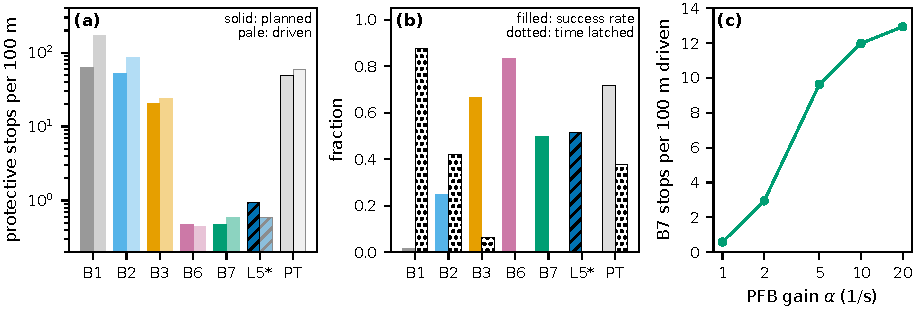
\includegraphics[width=\textwidth]{fig_journal_results.pdf}
\caption{Development-set (tuning-set) results. (a) Protective stops per 100\,m planned (solid) and driven
(pale), logarithmic scale. (b) Success rate (filled) and share of time latched (dotted). (c) B7's stops
per 100\,m driven and the PFB's fallback steps against the gain $\alpha$. L5$^*$ is the pilot checkpoint of
seed 9000002 (hatched); PT is the privileged tracker (control).}
\label{fig:results}
\end{figure}

Table~\ref{tab:main} and Figure~\ref{fig:results} summarise the development set. Placing the PFB beneath
the tuned RPP planner reduces its protective stops from 52.8 to 0.47 per 100\,m planned (86.1 to 0.59 per
100\,m driven) and the time spent latched from 42\,\% to 0.05\,\%, while the success rate rises from 0.25
to 0.50. The reduction holds in every stratum, with no stop in the narrow and medium aisles
(Table~\ref{tab:strata}).

\begin{table}[!htbp]
\centering
\caption{RPP without (B2) and with (B7) the PFB by clearance stratum; development set, 20 scenarios per
stratum; stops per 100\,m driven.}
\label{tab:strata}
\small
\begin{tabular}{lcccc}
\toprule
& \multicolumn{2}{c}{Success rate} & \multicolumn{2}{c}{Stops per 100\,m driven}\\
\cmidrule(lr){2-3}\cmidrule(lr){4-5}
Stratum & B2 & B7 & B2 & B7\\
\midrule
Narrow & 0.30 & 0.40 & 59.4 & 0.0\\
Medium & 0.15 & 0.40 & 88.7 & 0.0\\
Wide & 0.30 & 0.70 & 118.7 & 1.76\\
\bottomrule
\end{tabular}
\end{table}

\paragraph{Driving speed.} A filter could avoid stops simply by slowing the robot. On the 13 routes on
which B7 reached the horizon without meeting an obstacle, B7 and B2 move at the same speed outside stops,
0.057\,m/s pooled for both; B2 spends 27\,\% of these episodes latched and records 69 stops, B7 none. The
low speed of both is RPP's own: the tuned planner begins to regulate its speed at a clearance of 1.18\,m,
far above the clearance of any aisle, so it runs near its minimum speed throughout. In 10\,s in an empty
synthetic aisle the tuned RPP covers 0.73\,m, against 4.3\,m for Pure Pursuit and 4.2\,m for DWA. This is
a post-hoc observation on the development set.

\paragraph{Remaining failures of B7.} All 30 unsuccessful episodes end at the horizon, 28 of them without a
stop. In 17, an unmapped obstacle lies across the route; the privileged tracker fails exactly the same 17,
so no route follower that does not replan can complete them. B7's three stops occur in two of these
episodes: on retracing, they are preceded by steps on which no regime is feasible next to the obstacle,
and maximal braking does not keep the field clear. The other 13 failures are long routes (11.4--17.0\,m),
68--97\,\% complete at the horizon. On the 43 routes a route follower can traverse, B7 succeeds on 30.

\paragraph{The gain.} B7's success is nearly flat in $\alpha$ (0.50--0.52), because the horizon caps it,
whereas its stop rate rises monotonically from 0.59 to 12.9 per 100\,m driven (Figure~\ref{fig:results}c).
A smaller gain lets the barrier decay more slowly and keeps the robot further from the field, at the price
of more braking: at $\alpha=1$\,s$^{-1}$ the QP is infeasible on 332 steps, against 74 at
$\alpha=5$\,s$^{-1}$; at $\alpha\ge10$\,s$^{-1}$ the filter acts so late that fallback steps grow to
thousands. The selection fell on the low edge of the grid, which by the declared rule is reported and not
extended.

\paragraph{The classical references.} Pure Pursuit is non-functional under the certified fields: every one
of its 24 candidates completes at most one of 60 routes, latched 83--90\,\% of each episode. Five retraced
failures each end in an unrecoverable stop after six to eight stops at the same shelf corners, with the
route tracked to within 1--8\,cm: the failure is the interaction with the field and its restart
condition, not tracking. B2 fails 75\,\% of its routes by the same stop--recovery--restop cycle. DWA
reaches a higher success than B7 (0.667) at 20.5 stops per 100\,m planned. The field-aware MPPI planner,
which carries the certified band fields in its rollout cost, is the strongest reference: it succeeds on 50
of the 60 scenarios and records three stops. B6 and B7 are indistinguishable at 3 versus 3 events (0.47
per 100\,m planned each); the development set cannot separate them. The tuned B3 and B6 share their
sampler seed, so their candidate sets are not independent draws, and B6's smoothness weight and B3's
clearance weight lie at 93\,\% of their logarithmic ranges; both are disclosed.

\subsection{Learned planners: pilot results}\label{sec:res-learned}

\begin{table}[!htbp]
\centering
\caption{G4 pilot gate of the learned arms. Pilot seeds never enter the confirmatory analysis. Learning:
success over the last 10\,\% of training episodes (all on the full distribution); checkpoint: success of
the deterministic policy on the 60 tuning scenarios. Controls sound in every gate (zero action 0/60;
privileged tracker 43/60).}
\label{tab:g4}
\small
\begin{tabular}{llcccl}
\toprule
Arm & Pilot seed & Steps & Learning & Checkpoint & Verdict\\
\midrule
L1 & 9000000 & $3\times10^5$ & 0.00 & 0/60 & fail (pre-amendment rules)\\
L1 & 9000001 & $2\times10^6$ & 0.006 & 1/60 & fail\\
L1 & 9000002 & $2\times10^6$ & 0.061 & 0/60 & fail\\
L5 & 9000001 & --- & --- & --- & integrity failure, not counted\\
L5 & 9000002 & $2\times10^6$ & 0.463 & 31/60 & \textbf{pass}\\
L5 & 9000003 & $2\times10^6$ & \pending[running] & \pending[running] & \pending[running]\\
L2 & 9000002 & $2\times10^6$ & \pending[running] & \pending[running] & \pending[running]\\
L4 & 9000002 & $2\times10^6$ & \pending[running] & \pending[running] & \pending[running]\\
\bottomrule
\end{tabular}
\end{table}

Table~\ref{tab:g4} gives the pilot gates. The shaped, unfiltered planner L1 failed on all three pilot
seeds. Its first seed, under the original budget of $3\times10^5$ steps, completed 75 episodes, none
successful, 51 of them ending in unrecoverable stops; the learning setup was then changed once, identically
for every learned arm, before any confirmatory run (a $2\times10^6$-step budget, the curriculum and the
stall truncation), and the proximity weight was re-derived (Section~\ref{sec:methods}). Under the new
setup L1 still failed twice, with training success near 0.1 or below and a late dip at the same point in
both seeds; its deterministic checkpoints completed one and zero routes of 60. By the declared rules L1 trains its confirmatory seeds
regardless, and its failures are disclosed: a non-learning comparator is an easy one, and the weight of H1
rests on L2 and B6.

The filtered planner L5 passed G4 on its first counted pilot seed (its earlier seed ended in a crash
caused by a defect in the filter's restart check, fixed under amendment and not counted as a gate
failure). Its training completed 924 of 1{,}754 episodes with no unrecoverable stop; its last-decile
success was 0.463, and its deterministic checkpoint succeeded on 31 of 60 tuning scenarios (narrow 6/20,
medium 11/20, wide 14/20) with 29 timeouts, no unrecoverable stop and no contact. It recorded six stops:
0.95 per 100\,m planned, 0.59 per 100\,m driven (Table~\ref{tab:main}). The pivot to \Hprime\ was not
triggered.

\paragraph{The learned planner leans on the filter.} Offline diagnostics on the pilot checkpoint, without
training, found no defect but two behaviours that matter for interpretation. First, the PFB alters L5's
command on essentially every step, including in episodes that follow the route closely and succeed. The
policy requests near-maximal planar speed (median 0.43--0.63\,m/s in five of six traced episodes, with
45--99\,\% of steps at or above 0.45\,m/s) while it moves at 0.13\,m/s: the filter sets the speed, the
policy mostly the direction. B7's RPP, by contrast, requests 0.07\,m/s and is altered on 50--89\,\% of steps
in its two traced episodes. Second, L5 \emph{wanders}: it drives 1.6 times the planned length of its
routes (narrow 1.73, medium 1.45, wide 1.61). In every traced case this is a smooth, deterministic detour
of 4--6\,m over open floor around the racks in narrow-aisle routes, accruing while route progress stalls,
mostly near the route's end, without oscillation (with one exception), goal overshoot or circling; the
stochastic and deterministic policies wander alike. The wandering is why the primary endpoint divides by
planned rather than driven length: per 100\,m driven, L5 (0.59) ties B7, whereas per 100\,m planned it
records twice the rate of B6 and B7. Its rare stops occurred with the filter active and no fallback,
consistent with prediction lag or estimation error rather than infeasibility.

\subsection{Computational cost}
On the training host (one desktop GPU workstation, four simulator instances running), the 95th percentile
of the per-step decision time was 27.9\,ms for the PFB's QP within B7 (median 1.6\,ms, maximum 49.5\,ms),
28.0\,ms within L5, 34.5\,ms for B6 in situ (37.1\,ms in a synthetic measurement) and below 2.5\,ms for B1
and B2 including their route cap and recovery. All lie within the 50\,ms control period. These figures are
descriptive; no compute advantage over B6 is claimed. Training L5 with the filter in the loop ran at 21.1
steps/s per instance, against about 33 steps/s for the unfiltered L1.

\subsection{Held-out evaluation}
Tables~\ref{tab:h1} and~\ref{tab:h2} are reserved for the preregistered evaluation on the test set. They
will be filled from a single test evaluation after the confirmatory seeds are trained.

\begin{table}[!htbp]
\centering
\caption{Reserved: H1 and \Hprime\ on the unmapped-static test condition, strata pooled. Rate ratio of
protective stops per 100\,m planned with its two-level interval at the Holm level; success and mission time
descriptive. \textbf{Held-out evaluation pending.}}
\label{tab:h1}
\small
\renewcommand{\pending}{\textcolor{red}{[pending]}}
\begin{tabular}{lcccc}
\toprule
Comparison & SP100 (comparator) & Rate ratio [CI] & Success & Mission time (s)\\
\midrule
L5 vs B1 & \pending & \pending & \pending & \pending\\
L5 vs B2 & \pending & \pending & \pending & \pending\\
L5 vs B3 & \pending & \pending & \pending & \pending\\
L5 vs B6 & \pending & \pending & \pending & \pending\\
L5 vs L1 & \pending & \pending & \pending & \pending\\
L5 vs L2 & \pending & \pending & \pending & \pending\\
L5 vs L3 & \pending & \pending & \pending & \pending\\
\midrule
B7 vs B1 (\Hprime) & \pending & \pending & \pending & \pending\\
B7 vs B2 (\Hprime) & \pending & \pending & \pending & \pending\\
B7 vs B6 (\Hprime) & \pending & \pending & \pending & \pending\\
\bottomrule
\end{tabular}
\end{table}

\begin{table}[!htbp]
\centering
\caption{Reserved: H2, narrow-stratum success of L5 and L4, both test conditions pooled and each separately.
\textbf{Held-out evaluation pending.}}
\label{tab:h2}
\small
\renewcommand{\pending}{\textcolor{red}{[pending]}}
\begin{tabular}{lccc}
\toprule
Condition & L5 & L4 & Difference [CI]\\
\midrule
Pooled & \pending & \pending & \pending\\
Mapped-only & \pending & \pending & \pending\\
Unmapped-static & \pending & \pending & \pending\\
\bottomrule
\end{tabular}
\end{table}

%=====================================================================================================
\section{Discussion}\label{sec:discussion}

\paragraph{Consistency with the certified field.} On the development set, a barrier whose safe set is the
complement of the certified trigger set removed almost all protective stops of an unmodified classical
planner, in every stratum, without slowing it. The point of the construction is that the filter need not
be tuned against the safety equipment: it is as conservative as the equipment, by sharing its field, and
any residual stop has a nameable cause (infeasibility next to an obstacle across the route, prediction
error). The gain $\alpha$ then trades stops against braking, not against throughput, within the range
tested.

\paragraph{A filter beneath a planner, or a planner that knows the field.} The field-aware MPPI planner B6
reached as few stops as B7, with a higher success rate, by carrying the same kind of field in its cost. The
two approaches are indistinguishable at 3 versus 3 events, and their relative merit for stops, success and
compute is the subject of the held-out evaluation. They differ in what they require: B6 replaces the
planner and spends most of a control period sampling, whereas the PFB is a layer beneath a planner that has
no knowledge of the field. The approaches are complementary rather than exclusive; a field-aware planner
above the PFB is a natural next step.

\paragraph{The learned planner leans on the filter.} L5 is defined as the policy with the filter in the
loop, and it has learned to use it: it asks for the maximum speed and lets the filter regulate speed,
keeping the direction. This is not a defect of the method, but it bears on what the method is. The
learned component contributes routing and direction; the safety-relevant regulation is the filter's. It
also makes the intervention penalty of \eqref{eq:reward} a weak incentive in practice. Whether a stronger
incentive, or a policy that observes the field, yields a policy that needs less correction is an open
question outside the declared design, which forbids changing the reward between pilot and confirmatory
training.

\paragraph{Wandering and the choice of denominator.} The learned planner's detours over open floor made a
rate per distance driven flattering to it and unflattering to planners that time out short of the goal.
Dividing by planned length removes the incentive and is conservative for L5 (0.59 becomes 0.95 per
100\,m). The detours themselves point to a limitation of the learned local planner without replanning: in
narrow aisles it sometimes prefers to go around the racks.

\paragraph{Weak classical references.} B1 cannot complete routes under the certified fields with any of its
tuned parameters, and B2 fails most routes in a stop--recovery--restop cycle; both are the status quo of
route trackers that rely on the scanners, and comparisons against them are easy. The informative
comparisons are against B3 and, above all, B6. B2's tuned proximity regulation also makes B7 slow, which
the 200\,s horizon turns into timeouts; that is a property of the tuned RPP, inherited by B7 by design
(B7 reuses B2's parameters), not of the filter.

\paragraph{Limitations.} The evidence is subject to several limitations. (i) Every number is a
development-set result on 60 scenarios with few events for the strongest arms; parameters and $\alpha$ were
selected on the same set. (ii) Learned results come from one passing pilot seed and three failing ones;
seed-to-seed variance is not yet measured, and the power analysis shows that H1 may end inconclusive at
plausible rates. (iii) The study is simulation-only, on one platform, conditioned on the ODE engine; the
velocity estimate uses the simulator's ground-truth pose; obstacles below the single scan plane are unseen.
(iv) The certified layer is an emulation with three speed bands, more conservative than typical
installations in some respects (worst-case acceleration through the response time, rotation sweep) and
kinder in one (the automatic receding release); no certification claim is made for the emulator, the
filter or the sensing. (v) Classical planners receive a recovery behaviour and a route speed cap that
learned planners do not. (vi) The PFB's trust interval and band speed margin were set on tuning routes to
remove observed failures, and $\alpha$ lies on the edge of its grid. (vii) Obstacles are static; moving
people, the main reason protective fields exist, are not modelled.

%=====================================================================================================
\section{Conclusion}\label{sec:conclusion}

The Protective-Field Barrier is a control barrier function whose safe set is taken from the certified
safety function it sits above: the complement of a continuous protective field built from the footprint,
the speed, the direction and the yaw rate of a holonomic robot. One QP per speed regime minimally corrects
the command of an arbitrary planner within the base's limits. On the development set it removed almost
all protective stops of a tuned classical planner without slowing it, and a reinforcement-learning planner
trained with it in the loop passed its pilot gate where a shaped planner without it did not. These are
preliminary results. The confirmatory comparisons, the declared exploratory contingency \Hprime\ and the
learned arms' confirmatory seeds will be evaluated once, on held-out layouts, under the preregistered
analysis; until then, the claims of this draft are limited to what the development set and the pilots can
show. Future work includes field-aware planners above the filter, moving obstacles, and the transfer to a
physical vehicle with certified scanners.

\section*{Data and code availability}
\tbd{Repository link for code, scenario sets and run data, or a statement of availability, to be decided
by the authors.}

\section*{Acknowledgements}
\tbd{Funding and acknowledgements. Generative-AI disclosure as required by the chosen venue: tool, version
and purpose of use.}

\bibliographystyle{plainnat}
\bibliography{references}

%=====================================================================================================
\appendix
\section{Notation}\label{app:notation}

\begin{table}[h]
\centering
\small
\begin{tabularx}{\textwidth}{lXl}
\toprule
Symbol & Meaning & Value\\
\midrule
$\Delta t$ & control period & 0.05\,s\\
$\mathbf{u}=(v_x,v_y,\omega)$ & body command & ---\\
$\mathbf{u}^{\mathrm{nom}},\mathbf{u}^-,\mathbf{u}^{\mathrm{app}}$ & nominal, previous applied, applied command & ---\\
$\hat{\mathbf{v}}$ & estimated body velocity & low-pass 0.10\,s\\
$\rho_{\mathrm{out}}$ & circumscribed radius of the footprint & 0.3374\,m\\
$L$, $v_{\mathrm{rim}}$, $f$ & lever arm; rim-speed ceiling; filter share & 0.3865\,m; 0.617\,m/s; 0.95\\
$a_{\max},a_{\mathrm{dec}},\alpha_{\max}$ & limiter bounds & 0.5, 1.0\,m/s$^2$; 1.4\,rad/s$^2$\\
$t_r$, $T$, $t_d$ & response time; reach time; restart delay & 0.10, 0.15, 2.0\,s\\
$a_b$ & braking assumed by the fields & 1.0\,m/s$^2$\\
$V_\ell$ & band tops & 0.10, 0.30, 0.51\,m/s\\
$v_{\mathrm{cap}}$ & largest reachable planar speed & 0.5074\,m/s\\
$h(n)$, $\rho(\psi)$ & field support function; boundary distance & 1{,}440 normals\\
$S,E,D,\sigma,K,R$ & sweep, heading reach, travel depth, swerve, turning drift, at-rest reach & $E(0)=0.0315$\,rad, $R=0.0131$\,m\\
$m_f,m_l$ & margin ahead; abeam, behind and at rest & 0.10, 0.05\,m\\
$(r_k,\psi_k,\chi_k)$ & filter-stream sector: range, bearing, validity & $k=1,\dots,120$\\
$\lambda$ & regime: rest or band 0, 1, 2 & ---\\
$h^\lambda_k$, $g^\lambda_k$ & barrier now; predicted barrier & ---\\
$\tau,\tau_\ell$ & prediction horizon; lag allowance & 0.10, 0.05\,s\\
$M,\epsilon_\mu$ & realised fractions of the step; grid margin & $\{0,\frac14,\frac12,\frac34,1\}$; 0.5\,mm\\
$\delta$ & scan residual (binning penalty) & 0.5\,mm\\
$\alpha$ & class-$\mathcal{K}$ gain & 1.0\,s$^{-1}$ (frozen)\\
$k_p,c_t,k_{\mathrm{stop}},k_{\mathrm{int}},k_{\mathrm{prox}}$ & reward weights & 5, 0.01, 5, 0.1, 0 (L1, L4: 0.10113)\\
SP100 & protective stops per 100\,m of planned route & ---\\
\bottomrule
\end{tabularx}
\end{table}

\section{Verification findings}\label{app:verification}
Verification before training uncovered defects that would each have biased a safety evaluation silently.
We summarise them because they bear on any simulation study of protective stops.

\paragraph{Contact-check gaps.} The ground-truth contact check first watched the chassis only, while the
wheels stand about 17\,mm proud of it laterally; their contact shapes were not even collidable. Contact is
now the union of chassis and wheel checks, and a gate with six positive cases (including a raised obstacle
meeting a scanner housing above the chassis) and a 10\,mm negative case passes in the gate script and in
the environment's step loop.

\paragraph{A blind zone inside the protective field.} The platform's original centreline sensors left a
region beside the robot seen by neither; the scanner reported it free, because it judged validity by
bearing from the body origin. Every scanner check had placed its walls at 0.6\,m or more, just outside the
gap. Validity is now computed from each sensor's position with occlusion, and the corner layout was
adopted; a dense post sweep found every one of 7{,}680 cells observed (Figure~\ref{fig:coverage}).

\begin{figure}[h]
\centering
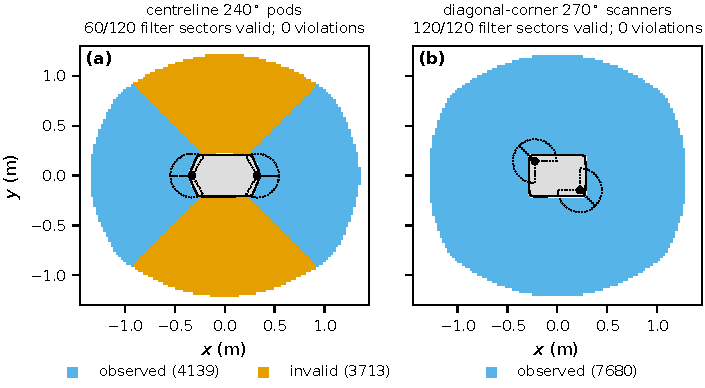
\includegraphics[width=0.85\textwidth]{fig3_coverage.pdf}
\caption{Sensor coverage by the dense post sweep (20\,mm post, 25\,mm grid, from the footprint edge to
1.0\,m beyond it), filter stream. (a) The original centreline layout: cells beside the robot are flagged
invalid, never reported free. (b) The adopted corner layout: every cell observed.}
\label{fig:coverage}
\end{figure}

\paragraph{A measurement that measured the wrong thing.} A 9.6\,mm ``scan penalty'' that justified a
clearance buffer turned out to be the test walls' half-thickness, since a cuboid is placed by its centre; a
positive control found it, and the real residual is $-0.27$ to $+0.50$\,mm. Every probe now carries a
positive control.

\paragraph{Corrections to the field and the restart.} The at-rest field was larger abeam than the moving
fields, so the field shrank as speed rose; rotation was not in the field; the field was sized for constant
motion rather than the motion reachable within the response time; stops did not nest; and release could
retrigger at once. Each was found by a test or a trace, ruled before implementation, recorded by
amendment, and is now guarded by a test.

\paragraph{Scan corruption under load.} A gate control requesting zero motion recorded a stop with the
robot stationary. A declared rerun reproduced it only under heavy CPU load: corrupted renders with most
sectors empty and phantom returns near the scanner corners. Because the filter adds compute per step, the
fault would have biased the comparison against filtered methods. The plausibility check, re-rendering and
fail-safe now handle it, and scan-fault stops are excluded from the primary count and reported.

\paragraph{Floor extent and placement.} Halls placed around a scenario's start reached 14.5\,m from the
origin on a floor that ended at 7.5\,m, and episode resets placed each hall around the previous episode's
end pose; both were fixed before any training, and a test now checks every built world against the floor.

\end{document}
